\pagestyle{fancy}
\chapter{RAG}  
\label{chap:RAG}  
This chapter explores Retrieval-Augmented Generation (RAG), which enhances Large Language Models (LLMs) by integrating retrieval from Vector Databases (VDBMSs) to mitigate their limitations. We discuss alternative RAG approaches, including Agentic RAG, which leverages AI agents for iterative reasoning and refinement.


\section{Retrieval-Augmented Generation}  
Large Language Models (LLMs) are trained on vast datasets, but they face challenges when queried about information beyond their training data. In such cases, they may either admit a lack of knowledge or, worse, generate inaccurate responses—a phenomenon known as hallucination. 

LLMs, despite their capabilities, have two significant limitations:  
\begin{itemize}  
    \item They can confidently produce incorrect or outdated information (hallucinations).  
    \item They may not have been trained on the specific data required for a given query.  
\end{itemize}  


Retrieval-Augmented Generation (RAG) addresses this issue by supplementing LLMs with relevant external data. Instead of relying solely on pre-trained knowledge, RAG retrieves pertinent documents and incorporates them into the prompt, ensuring more accurate and context-aware responses. This approach is sometimes referred to as generative search or in-context learning.  

RAG mitigates these issues through a two-step process:  
\begin{enumerate}  
    \item \textbf{Retrieval} – Relevant information is fetched based on a query.  
    \item \textbf{Generation} – The LLM is then prompted with both the retrieved data and the user's query, allowing it to generate a response using up-to-date and relevant information.  
\end{enumerate}  

By leveraging retrieval-based augmentation, RAG enhances the accuracy and reliability of LLM outputs, reducing reliance on potentially outdated or incorrect pre-trained knowledge.



\section{Agentic Retrieval-Augmented Generation (RAG)}

Retrieval-Augmented Generation (RAG) enhances Large Language Models (LLMs) by incorporating external knowledge, improving accuracy, and reducing hallucinations. Instead of relying solely on the static knowledge encoded during pretraining, RAG retrieves relevant information from external sources to provide more accurate, up-to-date, and contextually appropriate responses. 

However, traditional RAG approaches have several limitations:

\begin{itemize}
    \item \textbf{Static retrieval and generation process:} The retrieval step typically happens only once before the generation phase, which means there is no opportunity for iterative refinement based on context or response quality.
    \item \textbf{Limited to a single external knowledge source:} Most RAG implementations retrieve information from a single vector database (VDB), but some use cases require multiple sources, such as APIs, structured databases, or web-based knowledge repositories.
    \item \textbf{Lack of reasoning over retrieved information:} The retrieved context is used as-is without further validation, filtering, or iterative reasoning, potentially leading to the propagation of incorrect or incomplete information.
\end{itemize}

\subsection{Introducing Agentic RAG}
Agentic RAG extends the traditional RAG paradigm by introducing AI agents—autonomous LLM-based systems that perform specialized tasks while leveraging dynamic retrieval, reasoning, and tool use. Unlike standard RAG, which retrieves and applies context in a single step, agentic systems operate iteratively, refining their approach and responses through multiple retrieval and reasoning cycles.

In an agentic framework, each agent has a specific role, allowing for modular execution where tasks are divided and optimized at different stages. The agents operate in a structured, step-by-step manner, where each stage builds upon previous results, ensuring continuous improvement in response quality.

The key components of an AI agent include:

\begin{itemize}
    \item \textbf{LLM:} The core reasoning and generation engine responsible for processing information and making decisions.
    \item \textbf{Task:} A predefined objective or role assigned to the agent, guiding its execution strategy.
    \item \textbf{Long-term memory:} A persistent storage system, often implemented using vector databases (VDBMs), enabling the agent to retain learned information over multiple interactions.
    \item \textbf{Short-term memory:} A temporary state tracker that maintains context throughout execution, enabling dynamic workflow adjustments and information flow between agent interactions.
    \item \textbf{Tools:} External utilities such as APIs, databases, search engines, code execution environments, or computational functions that extend the agent's capabilities beyond text-based generation.
\end{itemize}

By leveraging these components, agents can actively retrieve, analyze, and refine information rather than passively relying on a single retrieval step. This iterative approach results in more contextually accurate and reliable responses.

\subsection{Agentic RAG and Agent-Based Frameworks}

Agentic RAG integrates agent-based frameworks with RAG, creating a dynamic pipeline that iteratively retrieves, reasons, and refines information. This approach addresses the limitations of static retrieval by enabling LLMs to interact with external tools, break down complex tasks, and continuously adapt based on intermediate results.

Unlike traditional RAG, which retrieves data once and directly uses it for generation, Agentic RAG incorporates multiple retrieval cycles, validation mechanisms, and step-by-step task execution. The agent can refine the retrieved information, cross-check responses, and adapt its approach dynamically.

Key characteristics of Agentic RAG include:

\begin{itemize}
    \item \textbf{Autonomous execution:} Agents execute tasks independently, continuously assessing and refining their output based on intermediate feedback.
    \item \textbf{Multi-step decision-making:} Instead of retrieving information once, agents can perform multiple queries, validate responses, apply logical reasoning, and adjust their strategy as needed.
    \item \textbf{Tool integration:} Agents leverage APIs, databases, and computational tools to dynamically fetch, analyze, and process external data beyond what is stored in their training corpus.
    \item \textbf{Dynamic adaptation:} Agents can modify their retrieval strategy based on contextual cues, ensuring more relevant and precise results.
    \item \textbf{Progressive refinement:} The agent iteratively improves responses by retrieving additional data, analyzing inconsistencies, and updating its understanding.
\end{itemize}

\section{Agentic Frameworks}

Agentic frameworks provide structured methodologies for developing AI agents that integrate reasoning, retrieval, and action execution. These frameworks enable the creation of more intelligent and autonomous LLM-powered systems by allowing agents to dynamically interact with tools, retrieve external knowledge, and refine their responses iteratively. By leveraging these frameworks, developers can design AI agents that retrieve information more accurately, adapt dynamically to new inputs, and maintain context over extended interactions.


\subsection{ReAct Framework}

One widely adopted framework for agent-based reasoning is the ReAct framework, which stands for \textbf{Reason + Act}. A ReAct agent processes sequential, multi-step queries while maintaining state by combining reasoning, tool use, and query planning into a cohesive workflow.

The ReAct process follows an iterative cycle:

\begin{itemize}
    \item \textbf{Thought:} Upon receiving a query, the agent reasons about the next action.
    \item \textbf{Action:} The agent executes the decided action, such as querying a database, calling an API, or retrieving relevant documents.
    \item \textbf{Observation:} The agent evaluates the output of the action and determines the next step.
\end{itemize}

This cycle repeats until the agent reaches a final response. The iterative nature of ReAct allows it to refine answers dynamically, validate retrieved information, and adjust its approach based on real-time observations.

\subsection{LangChain and LangGraph}

Several frameworks have emerged to facilitate the development of agentic systems, with \textbf{LangChain} and \textbf{LangGraph} being two of the most prominent. While both are designed to enable LLM-powered applications, they differ in their execution models and capabilities.

\subsubsection{LangChain: Modular and Sequential Execution}

LangChain provides a modular architecture for integrating LLMs with various external tools, databases, and APIs. It offers structured workflows for chaining multiple components, such as prompt templates, memory modules, and tool interfaces.

Key characteristics of LangChain:
\begin{itemize}
    \item \textbf{Sequential Execution:} LangChain primarily follows a linear pipeline, where tasks are executed in a predefined order.
    \item \textbf{Memory Management:} It supports both short-term and long-term memory, enabling persistent context handling across interactions.
    \item \textbf{Tool Integration:} LangChain allows agents to interact with APIs, databases, and custom functions, expanding their ability to fetch and process information.
    \item \textbf{Pre-built Components:} Developers can leverage pre-configured templates for common use cases, simplifying implementation.
\end{itemize}

LangChain is well-suited for structured LLM applications, such as chatbots, document retrieval systems, and structured automation pipelines, where execution follows a predictable sequence.

\subsubsection{LangGraph: Graph-Based Execution for Agentic Systems}

LangGraph extends LangChain by introducing a \textbf{graph-based execution model}, allowing agents to perform dynamic, non-linear reasoning and iterative refinement. Unlike LangChain’s sequential structure, LangGraph enables flexible workflows where execution can be cyclic, conditional, or parallel.

Key differences of LangGraph:
\begin{itemize}
    \item \textbf{Graph-Based Workflow:} Instead of a linear pipeline, LangGraph represents tasks as nodes and execution logic as edges, enabling more complex task decomposition.
    \item \textbf{Cyclic Execution:} Supports iterative reasoning, allowing agents to refine responses through multiple retrieval and validation steps.
    \item \textbf{Conditional Logic:} Agents can make real-time decisions based on retrieved information, enabling adaptive responses.
    \item \textbf{Multi-Agent Coordination:} Facilitates communication between multiple agents, each specialized for different tasks, improving efficiency in complex workflows.
\end{itemize}

LangGraph is particularly useful for applications requiring multiple retrieval steps, adaptive decision-making, and real-time processing, such as dynamic research assistants, financial analysis bots, and multi-agent orchestration systems.

\subsection{Example of Document Retrieval with LangGraph}
As previously mentioned, Agentic RAG helps overcome the limitations of static RAG. One such improvement can be observed in the following experiment. The initial setup consists of a vector database containing PubMed documents indexed using an HNSW index. Each document includes a title, abstract, and tags, all of which are embedded using the multilingual Ollama model. The challenge arises during querying: when searching for documents related to \textit{breast cancer}, the vector database embeds the query, retrieves the top $K$ matching documents, and forwards them to the LLM for response generation. However, if an irrelevant but semantically similar document (such as documents about mouth cancer or cancer in general) is included in the retrieved set, the LLM may produce suboptimal results due to the presence of non-relevant context.

\begin{figure}[h]
    \centering
    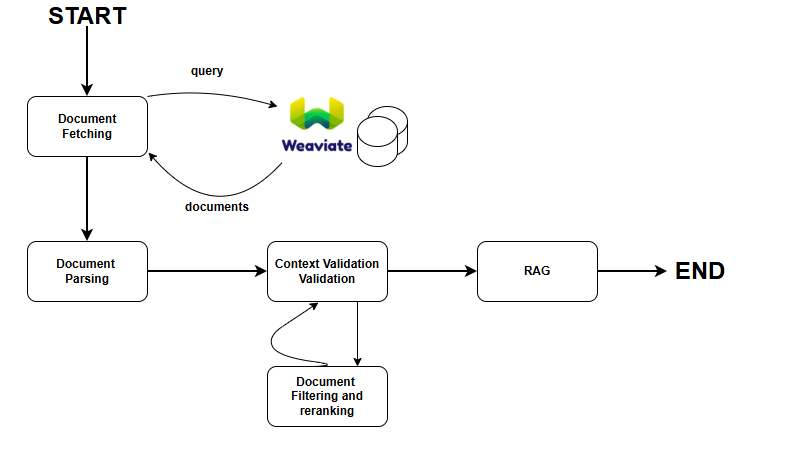
\includegraphics[width=0.8\textwidth]{IMAGES/immagine_2025-03-22_165130054.png}
    \caption[LangGraph Workflow]{LangGraph Workflow for Document Retrieval.}
\end{figure}


LangGraph addresses this issue by introducing a structured, step-by-step retrieval process where each agent performs a distinct task. These tasks include:
\begin{itemize}
    \item Fetching documents from the vector store
    \item Parsing the vector database output
    \item Validating the retrieved context using an LLM
    \item Correcting and re-ranking the context
    \item Providing the refined context to the LLM
\end{itemize}
This structured approach significantly enhances the RAG workflow by ensuring more accurate results while also standardizing the retrieval process.

\chapter{GraphRAG}
This chapter introduces the concept of Retrieval-Augmented Generation (RAG) in conjunction with Knowledge Graphs, which serve as structured data representations that capture complex relationships between entities. Knowledge Graphs are particularly advantageous due to their ability to synthesize information and reveal intricate connections between data points, making them an effective tool for enhancing retrieval-based AI models. We begin by exploring the applications of Graph RAG, demonstrating how it improves information retrieval by leveraging structured data. Following this, we delve into the core experiment of this thesis: the implementation of an Agentic RAG system that utilizes a Knowledge Graph to represent relational database schemas. This innovative approach enables efficient graph traversal for SQL query generation, enhancing both the explainability and accuracy of the generated queries.

\section{Knowledge Graphs and GraphRAG}
Another RAG approach that has been lately gaining traction employs the graph based data structures known as Knowledge Graphs. These structures are particularly useful for representing entities as nodes and the relationships between them with edges.
\begin{figure}[h]
    \centering
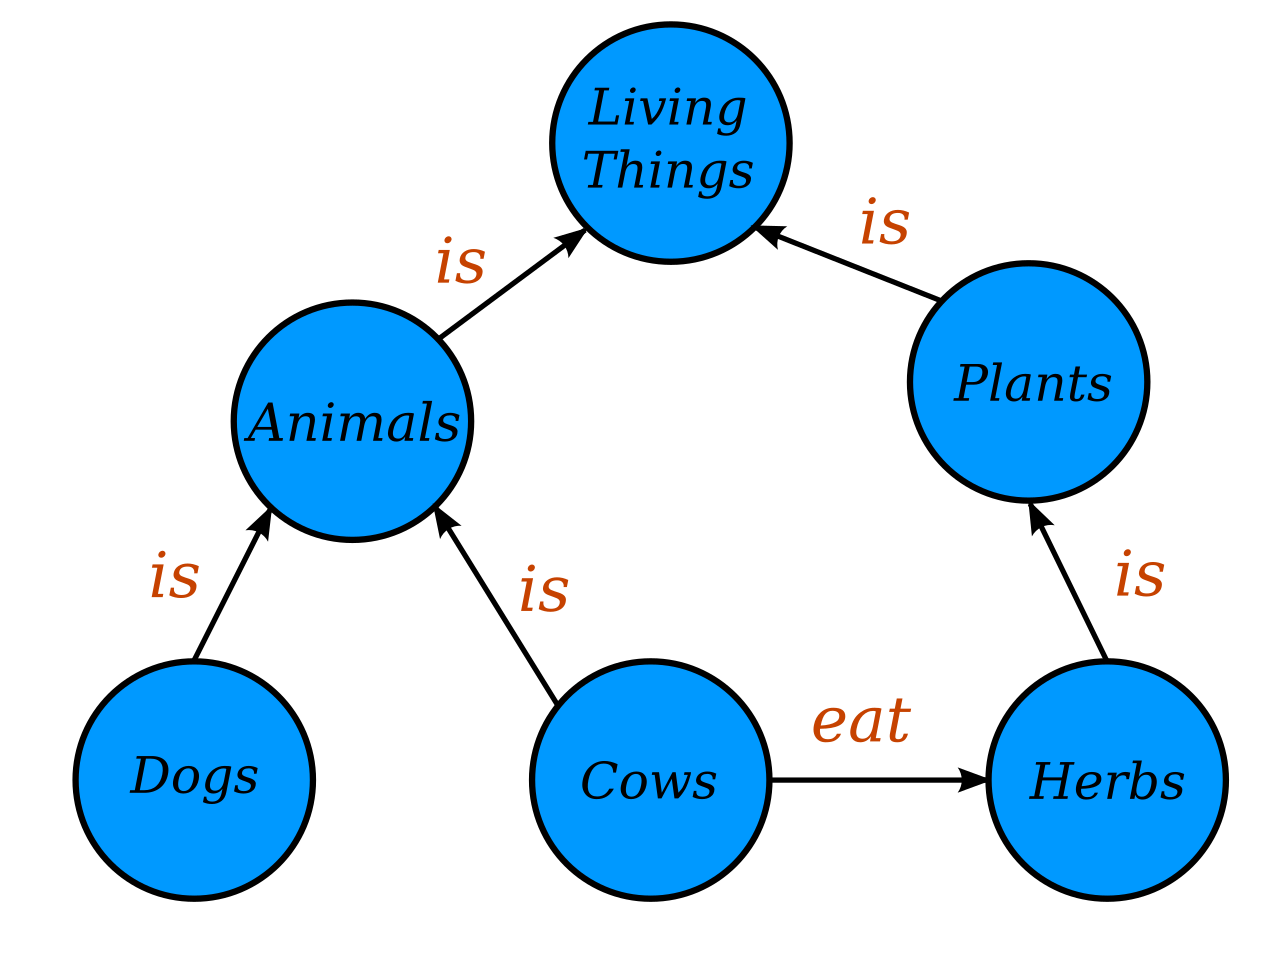
\includegraphics[width=0.65\textwidth]{IMAGES/Conceptual_Diagram_-_Example.svg.png}
    \caption[Knowledge Graph]{Example of Knowledge Graph. Source: Wikipedia\footnotemark}
    \label{fig:Knowledge Graph}
\end{figure}
\footnotetext{\url{https://en.wikipedia.org/wiki/Knowledge_graph}}
These graphs are widely used in AI-driven applications to enhance contextual understanding and reasoning by encoding explicit relationships between concepts. By structuring information in this way, knowledge graphs enable more sophisticated retrieval mechanisms beyond simple keyword or embedding-based searches. 

\subsection{GraphRAG: A Knowledge Graph-Driven RAG Approach}
In the context of Retrieval-Augmented Generation (RAG), knowledge graphs provide an alternative to traditional vector-based retrieval by making us of the more meaningful connections between concepts. While Vector based RAG systems rely on dense vector embeddings to find semantically similar text snippets, while being an effective technique is struggles with the sense making tasks that require understanding the relationships between entities across an entire dataset.

\subsection{Key Differences Between GraphRAG and Vector RAG}
The primary distinction between GraphRAG and Vector RAG lies in their retrieval mechanisms and capacity for global reasoning:

\begin{itemize}
    \item 	\textbf{Retrieval Mechanism:} Vector RAG uses embedding similarity to find relevant item, whereas GraphRAG navigates structured relationships within a knowledge graph.
    \item 	\textbf{Sensemaking Ability:} GraphRAG excels at answering global questions that require synthesizing information across multiple documents, while Vector RAG is better suited for fact-based, localized retrieval.
    \item 	\textbf{Scalability and Efficiency:} While GraphRAG requires an initial indexing phase to construct the knowledge graph, it can efficiently retrieve high-quality summaries for complex queries without retrieving an excessive number of items.
\end{itemize}


\subsection{Examples of Graph RAG  applications with LangChain}

With LangChain, we can provide a robust framework for integrating LLMs with our graph database by dynamically generating Cypher queries based on user questions. LangChain promotes seamless interaction between LLMs and graphs through the following components:

\begin{itemize}
    \item \textbf{Graph Database:} A structured representation of knowledge, such as Neo4j, where entities and relationships are stored.
    \item \textbf{Prompt Engineering:} A carefully crafted prompt template to guide the LLM in generating precise Cypher queries.
    \item \textbf{Query Execution:} The generated Cypher query is executed against the Knowledge Graph to retrieve relevant information.
    \item \textbf{Response Synthesis:} The retrieved data is processed and formatted into a natural language response by the LLM.
\end{itemize}

\begin{figure}[h]
    \centering
    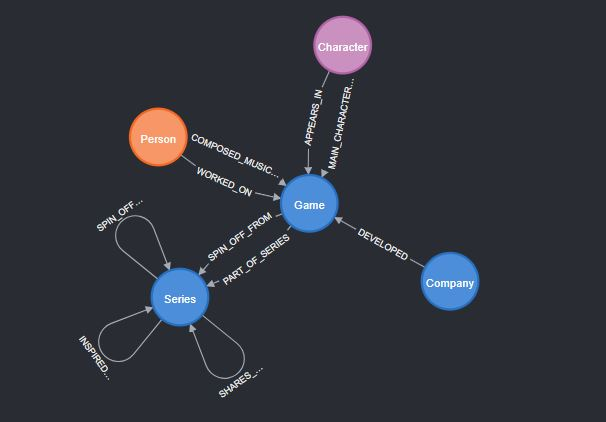
\includegraphics[width=0.9\textwidth]{IMAGES/Schema.JPG}
    \caption{KG schema visualized with APOC}
    \label{fig:Matching Nodes}
\end{figure}

In the figure above, we present a schema of our graph, which describes the entities related to game companies, the series produced, the people involved in game development, and even the characters. This serves as a heterogeneous knowledge base containing different types of entities connected to one another. 

For example, we can ask the LLM, \textit{"Which games has Kazuma Kaneko worked on?"} The chain responds with: \textit{"Kazuma Kaneko worked on Shin Megami Tensei III: Nocturne, Shin Megami Tensei V."} 


In the figure below, we illustrate the steps taken by LangChain:
\begin{figure}[h]
    \centering
    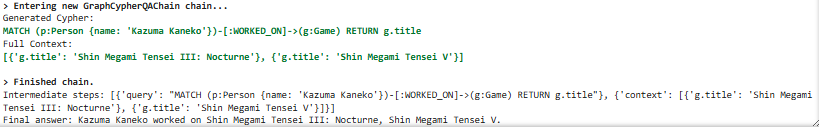
\includegraphics[width=1.1\textwidth]{IMAGES/immagine_2025-03-31_122504590.png}
    \caption{LangChain steps}
    \label{fig:Matching Nodes}
\end{figure}

Another angle worth exploring is the one about processing unstructured data into a Knowledge Graph. This way we can get the advantages of structured data such as finding complex relationships and patterns between entities, by starting from just a corpus of unstructured data. To construct this Knowledge Graph, LangChain leverages the use of an LLM that parses the text and categorizes the entities and their relationships. In the images below we can see the text corpus and the resulting schema of our generated Knowledge Graph.
\begin{figure}[h]
    \centering
    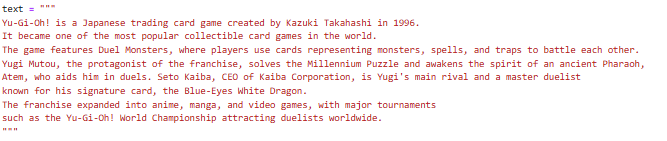
\includegraphics[width=1.1\textwidth]{IMAGES/immagine_2025-03-31_164059272.png}
    \caption{Text corpus}
    \label{fig:Matching Nodes}
\end{figure}
\begin{figure}[h]
    \centering
    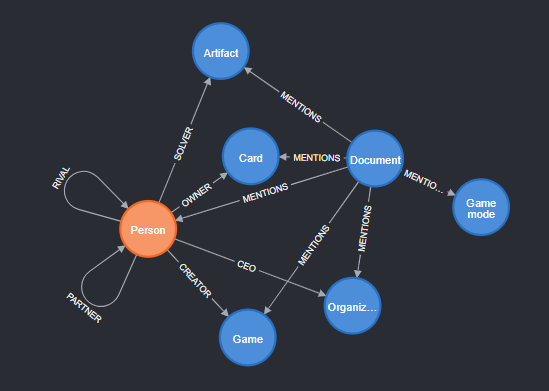
\includegraphics[width=0.7\textwidth]{IMAGES/immagine_2025-03-31_163821435.png}
    \caption{Generated Knowledge Graph}
    \label{fig:Matching Nodes}
\end{figure}


As demonstrated, LangChain effectively generates precise Cypher queries and retrieves relevant context from the Knowledge Graph to construct accurate responses. It is capable also of constructing Knowledge Graphs from unstructured data such as documents or corpus of text. However, while this approach is beneficial, it has limitations in handling more complex queries, and the still experimental nature of graph building dedicated LLMs, make it less suitable for production environments. A more adaptable solution for implementing Graph RAG is to utilize LangGraph, which enables greater control over workflow execution and allows for the incorporation of additional steps to improve response accuracy and handling of intricate queries.


\section{Experimental SQL generation with Knowledge Graphs}
In this final section, we present an experiment that integrates the theoretical principles discussed throughout this thesis. The experiment explores the use of Knowledge Graphs in generating SQL queries from natural language prompts. The workflow is built around LangGraph, which systematically processes natural language input to generate SQL queries. The process begins by constructing a Knowledge Graph from the schema of two CSV tables retrieved from the OpenData platform, which we will discuss shortly. This schema is represented as a Knowledge Graph in Neo4j, providing a structured understanding of the data relationships. LangGraph leverages a Large Language Model (LLM) to generate a Cypher traversal query, establishing connections between the two tables. The generated query then undergoes validation, ensuring it meets syntax requirements and other adequacy criteria before final execution.
\subsection{Workflow}

The general workflow of the architecture follows these steps:

\begin{enumerate}
    \item \textbf{Schema Analysis and Knowledge Graph (KG) Building}:  
    The CSV files are loaded, and a knowledge graph is constructed to represent the schema of the tables.

    \item \textbf{Vectorization and Storage}:  
    Column labels are vectorized and stored in a vector database, such as Weaviate, using Ollama.

    \item \textbf{Entity Matching}:  
    A two-step matching process is performed:  
    \begin{itemize}
        \item \textit{Label-Based Search}: Using cosine similarity to find relevant columns.  
        \item \textit{Value-Based Matching}: A customized scoring function evaluates whether columns can be joined based on their values.
    \end{itemize}

    \item \textbf{Schema Filtering}:  
    To improve Cypher query generation accuracy, schema elements irrelevant to the natural language question are filtered out. Only tables and relationships that exceed a predefined threshold are retained.

    \item \textbf{Question Enrichment}:  
    The natural language question is enriched with schema labels, reducing ambiguity and improving the mapping between the question and the schema for Cypher query generation.

    \item \textbf{Cypher Query Generation}:  
    A Cypher query is generated based on the enriched question and filtered schema.

    \item \textbf{SQL Generation}:  
    Finally, an SQL query is generated from the Cypher query.
\end{enumerate}


\subsection{Motivations}
Our experiment addresses the challenge of querying structured databases using natural language. Traditional database queries require structured syntax, such as SQL, which must adhere to the database schema and its constraints. However, users may not have full knowledge of the database structure—only a general understanding of the domain. Even with SQL expertise, writing accurate queries can be time-consuming and costly.  

To overcome these limitations, we propose a scalable framework that enables users to query databases using natural language while maintaining accuracy comparable to that of a data expert. This approach simplifies database interactions, reduces the need for deep schema knowledge, and enhances efficiency.

\subsection{Knowledge Graph Construction}
The \textbf{Knowledge Graph} serves as a structured data representation that captures entities and their relationships. The first step in the process is constructing the Knowledge Graph, where \textbf{tables and columns} are represented as \textbf{nodes}, and their relationships are defined by \textbf{edges}. Specifically, edges emphasize the association between columns and the tables they belong to.  

Additionally, column nodes include metadata such as:  
\begin{itemize}
    \item \textbf{Uniqueness} – to determine whether a column serves as an identifier.
    \item \textbf{Data type} – to ensure strict matching between columns of the same type, with the exception of cases where \textbf{float and integer} types may be considered compatible.
\end{itemize}

In the \textbf{Neo4j} graph, the possible relationships include:  
\begin{itemize}
    \item \textbf{"HAS COLUMN"} – an edge connecting a \textbf{table node} to its \textbf{column nodes}.
    \item \textbf{"SAME ATTRIBUTE"} – an edge linking \textbf{column nodes} that share the same label and metadata. However, if two columns match perfectly, instead of creating a relationship, they are \textbf{collapsed into a single node} to maintain data integrity.
\end{itemize}

By leveraging this \textbf{Knowledge Graph}, we enable traversals between columns that effectively represent \textbf{joins} between relational database tables.
\begin{figure}[h]
    \centering
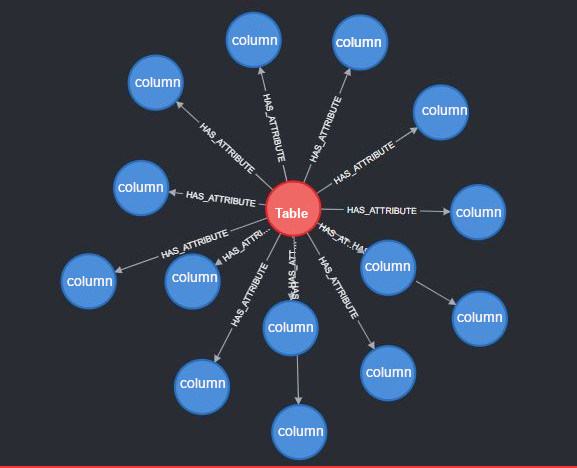
\includegraphics[width=0.7\textwidth]{IMAGES/KGschema.JPG}
    \caption{Example of generated Knowledge Graph}
    \label{fig:Knowledge Graph}
\end{figure}


\subsection{Entity Matching}
After constructing the Knowledge Graph, we also vectorize the column labels and store them in a Vector Database. For this, we use \textbf{Weaviate}, chosen for its lightweight processing, flexibility in vectorization, and ease of integration across platforms—thanks to its official \textbf{Docker} container. Weaviate supports multiple vectorization methods, and for this use case, we employ an \textbf{Ollama} container running the \textbf{snowflake-arctic-embed2} model, which provides fast and efficient lightweight vectorization.
\begin{figure}[h]
    \centering
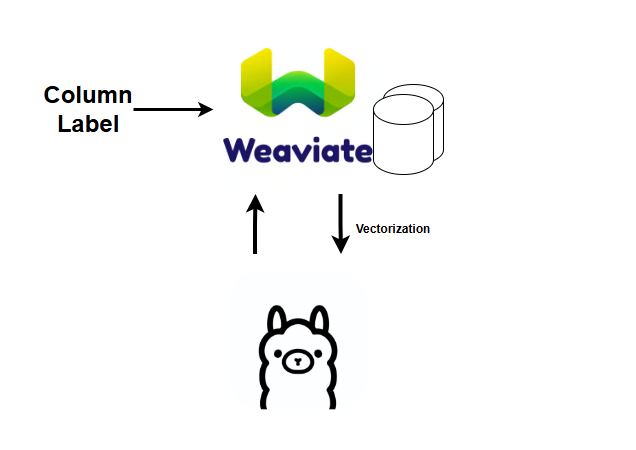
\includegraphics[width=0.65\textwidth]{IMAGES/immagine_2025-03-27_153710010.png}
    \caption{Column label vectorization}
    \label{fig:Vectorization}
\end{figure}
To store the vector embeddings, we use \textbf{Weaviate’s default flat index}, as the dataset contains only a few hundred embeddings. In this case, a flat search offers similar performance to \textbf{HNSW}, making it a practical choice for simplicity and efficiency.

Once the vector store is built, entity matching begins. Each column label undergoes a \textbf{vector search}, retrieving candidates with a similarity score above a predefined threshold. If a match meets this criterion, we perform a \textbf{value-based scoring} step to determine whether the columns are suitable for joining. A good join key should:

\begin{enumerate}
    \item \textbf{Have similar content} – The values should be closely related or directly matching.
    \item \textbf{Exhibit diversity} – Columns with excessive repetition (e.g., "Yes"/"No" or a single repeated category) provide little value in a join.
    \item \textbf{Share overlapping unique values} – Columns with entirely different value distributions are less useful for meaningful joins.
\end{enumerate}


The scoring process is based on a \textbf{TF-IDF vectorizer} provided by the \texttt{scikit-learn} library. The steps involved are as follows:

\begin{enumerate}
    \item The values within each column are vectorized using the TF-IDF method.
    \item A similarity matrix is computed, and the diagonal elements are extracted to calculate the mean similarity score.
    \item A penalty factor is applied to columns with a low diversity of unique values, reducing their overall score.
    \item The adjusted similarity score is compared against a predefined threshold to determine if the columns should be considered a match.
\end{enumerate}

If the similarity score exceeds the threshold, the Knowledge Graph is updated accordingly. The matched columns are linked via an edge labeled \textbf{"SAME ATTRIBUTE"}, which stores the computed similarity score as an edge property.
\begin{figure}[h]
    \centering
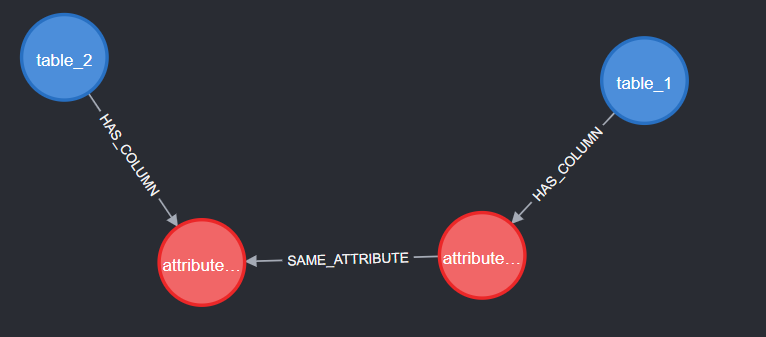
\includegraphics[width=0.7\textwidth]{IMAGES/immagine_2025-03-27_154727649.png}
    \caption{Example of matching nodes in the Knowledge Graph}
    \label{fig:Matching Nodes}
\end{figure}

\subsection{Schema Filtering and Question Enrichment}

After building the Knowledge Graph and Matching the entities, to enhance the accuracy of Cypher query generation, we introduce a two-step process: \textit{Schema Filtering} and \textit{Question Enrichment}.

\subsubsection{Schema Filtering}  
In this step, we refine the schema by filtering out elements that are not relevant to the given natural language question. Only tables and their traversals that meet a predefined relevance threshold are retained. This reduces noise and ensures that the generated Cypher query is based on the most pertinent schema components.The schema provides also similarity scores between nodes, this allows us to discern which column is needed to ensure the join statement.

\subsubsection{Question Enrichment}  
After schema filtering, the natural language question is enriched by incorporating schema labels and relationships between nodes. This step strengthens the connection between the question and the schema, reducing ambiguity and improving the precision of Cypher query generation. The expected resulting enriched prompt will contain the labels of the entities while still maintaining the sense of the original prompt.

\subsection{Cypher Generation with LangGraph Sub-Graphs}
For Cypher query generation, we leverage LangGraph's support for sub-graphs, enabling the construction of larger and more complex graphs in a modular manner. 
\begin{figure}[h]
    \centering
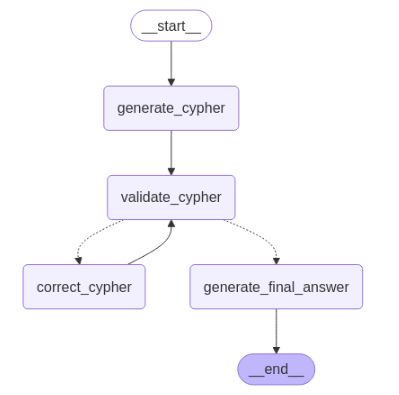
\includegraphics[width=0.55\textwidth]{IMAGES/LangGraph 2.JPG}
    \caption{Cypher Generation}
    \label{fig:Matching Nodes}
\end{figure}

The \textit{Cypher Generation} sub-graph begins with the provided enriched prompt and schema, generating the initial Cypher traversal. Once the traversal is created, an iterative process of validation and correction is employed to ensure the correctness of the query. 

To verify syntax accuracy, the query is executed using the \texttt{EXPLAIN} clause, which helps detect errors. Additionally, the process includes validating the existence of specific edges to ensure the correct generation of the Cypher query. Once validated, the final query is output to the main graph for further processing.


\subsection{SQL Translation from Cypher Traversal}

Once the Cypher query is generated, it provides a traversal that links table nodes through common neighbors, effectively representing the joining columns. This structured traversal serves as a bridge between the graph representation and relational databases, facilitating a seamless translation into SQL.

The SQL translation process closely mirrors the Cypher generation workflow, ensuring correctness through an iterative validation approach. Since the Cypher query already encodes the necessary relationships and joins, the translation primarily involves mapping graph-based traversals into equivalent SQL join operations. 

To guarantee syntactic accuracy, an iterative validation process is applied, similar to the validation performed during Cypher generation. This includes executing preliminary checks and leveraging SQL execution plans to detect potential syntax errors or logical inconsistencies. Any detected issues prompt refinements to the query before finalizing the SQL output. 

This structured approach ensures that the generated SQL query accurately reflects the intended data retrieval logic while maintaining correctness and efficiency.


\subsection{Execution over UK and Canadian OpenData}

After detailing the entire process, this section demonstrates its application to OpenData provided by Canada and the UK using SPARQL and CKAN. The UK dataset involves combining two CSV tables: one containing indicators of knee pain and the other related to varicose vein conditions. Once the Knowledge Graph (KG) is constructed, we observe that the provided code achieves the highest similarity score when joining tables within the filtered schema.

\paragraph{Nodes Representing Columns:}
\begin{itemize}
    \item \textbf{Procedure}  
        \begin{itemize}
            \item \texttt{data\_type}: string
            \item \texttt{is\_unique}: \texttt{False}
            \item \texttt{value}
            \item \texttt{similarity}: 0.9566
        \end{itemize}
    \item \textbf{Year}  
        \begin{itemize}
            \item \texttt{data\_type}: string
            \item \texttt{is\_unique}: \texttt{False}
            \item \texttt{value}
            \item \texttt{similarity}: 0
        \end{itemize}
    \item \textbf{AgeBand}  
        \begin{itemize}
            \item \texttt{data\_type}: string
            \item \texttt{is\_unique}: \texttt{False}
            \item \texttt{value}
            \item \texttt{similarity}: -2.6154
        \end{itemize}
    \item \textbf{ProviderCode}  
        \begin{itemize}
            \item \texttt{data\_type}: string
            \item \texttt{is\_unique}: \texttt{False}
            \item \texttt{value}
            \item \texttt{similarity}: 3.2149
        \end{itemize}
    \item \textbf{PostOpQReadmitted}  
        \begin{itemize}
            \item \texttt{data\_type}: int
            \item \texttt{is\_unique}: \texttt{False}
            \item \texttt{value}
            \item \texttt{similarity}: 1.9546
        \end{itemize}
    \item \textbf{VaricoseVeinPostOpQLeftFrontCount}  
        \begin{itemize}
            \item \texttt{data\_type}: int
            \item \texttt{is\_unique}: \texttt{False}
            \item \texttt{value}
        \end{itemize}
    \item \textbf{KneeReplacementPostOpQReadmitted}  
        \begin{itemize}
            \item \texttt{data\_type}: int
            \item \texttt{is\_unique}: \texttt{False}
            \item \texttt{value}
        \end{itemize}
    \item \textbf{KneeReplacementOKSPostOpQPredicted}  
        \begin{itemize}
            \item \texttt{data\_type}: float
            \item \texttt{is\_unique}: \texttt{False}
            \item \texttt{value}
        \end{itemize}
\end{itemize}
\linebreak 
\paragraph{Question Refinement:} \linebreak
\linebreak 
\linebreak  
Initially, the query posed was: 
\textit{"What is the average count of varicose vein post-op questions left front for knee replacement patients readmitted to hospital, by age band and provider code?"}  

The refined question, incorporating schema labels, is: \\ 
\textit{"What is the average \texttt{VaricoseVeinPostOpQLeftFrontCount} for \texttt{Procedure} 'Knee Replacement' patients with \texttt{PostOpQReadmitted} greater than 0, grouped by \texttt{AgeBand} and \texttt{ProviderCode}?"}  

This enrichment ensures greater specificity by aligning the query with structured schema elements.

\paragraph{Traversal and SQL Conversion:}
The Cypher traversal identifies the most optimal path between tables based on similarity scores, determining that the best route is through the \texttt{ProviderCode} node. 
The Cypher Traversal goes as follows:

\begin{figure}[h]
    \centering
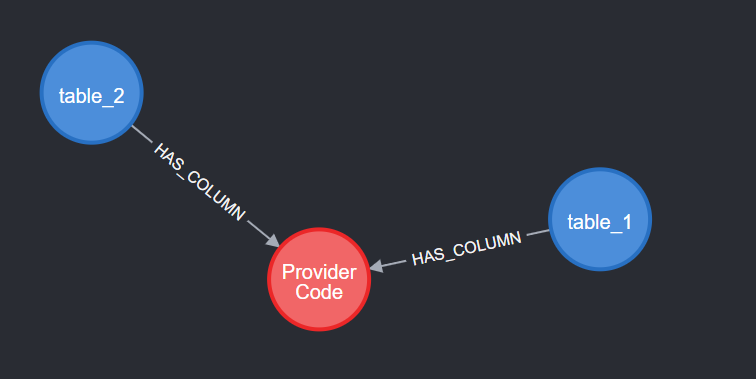
\includegraphics[width=0.65\textwidth]{IMAGES/immagine_2025-03-28_082503566.png}
    \caption{Generated Traversal}
    \label{fig:Traversal}
\end{figure}

This traversal is then converted into an equivalent SQL query:

\begin{verbatim}
SELECT T1.AgeBand, T1.ProviderCode, 
       AVG(T1.VaricoseVeinPostOpQLeftFrontCount) AS average_count
FROM Table1 T1
JOIN Table2 T2
ON T1.ProviderCode = T2.ProviderCode AND T1.AgeBand = T2.AgeBand
WHERE T2.PostOpQReadmitted IN (1, 'yes', TRUE, 'Yes') 
      AND T1.PostOpQReadmitted IN (1, 'yes', TRUE, 'Yes')
GROUP BY T1.AgeBand, T1.ProviderCode;
\end{verbatim}

\paragraph{Application to Canadian OpenData:}
For the query:  
\textit{"Get analysis types, values, and product types for Canadian samples"}  

The refined question becomes:  
\textit{"What are the \texttt{AnalysistypeTypedanalyse}, \texttt{ValuetextValeurtextuelle}, and \texttt{ProducttypeTypedeproduit} for samples from \texttt{CountryoforiginPaysdorigine} Canada?"}  

This results in the following SQL query:

\begin{verbatim}
SELECT DISTINCT 
    t1.AnalysistypeTypedanalyse AS analysis_type, 
    t1.ValuetextValeurtextuelle AS value, 
    t1.ProducttypeTypedeproduit AS product_type, 
    t2.AnalysistypeTypedanalyse AS analysis_type2, 
    t2.ValuetextValeurtextuelle AS value2, 
    t2.ProducttypeTypedeproduit AS product_type2
FROM Table1 t1
INNER JOIN Table2 t2 
ON t1.CountryoforiginPaysdorigine = t2.CountryoforiginPaysdorigine
WHERE LOWER(t1.CountryoforiginPaysdorigine) = LOWER('Canada') 
      AND LOWER(t2.CountryoforiginPaysdorigine) = LOWER('Canada');
\end{verbatim}

These examples illustrate how our methodology effectively refines user queries and generates precise SQL queries by leveraging Knowledge Graph-based enrichment.

\section{Join Discovery with a Knowledge Graph of \( N \) Tables}

Building upon the previously introduced job pipeline, we extend the process from joining two tables to handling a more complex use case involving \( N \) tables. The goal is to determine the necessary relational tables required for a given query. 
\subsection{Metadata Integration in the KG construction}
In this augmentation we keep the Knowledge Graph construction process mostly unchanged, aside from an additional step before the construction, which is fetching a sample of each CSV and instruct the LLM or a human operator to provide a brief description of what the relational table represents.This process is simple and straightforward making the difference between the performances of a human operator and a LLM minimal.
\begin{figure}[h]
    \centering
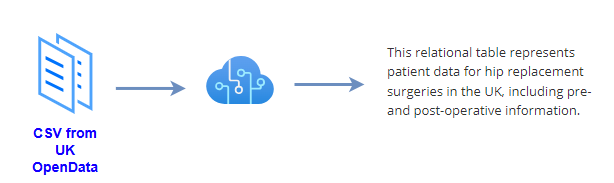
\includegraphics[width=0.65\textwidth]{IMAGES/immagine_2025-04-05_084400623.png}
    \caption{Example of an LLM's description of a Medical CSV}
    \label{fig:LLM CSV analysis}
\end{figure}


While the graph construction process remains almost unchanged, the primary modification occurs in the querying phase.
\subsection{Clustering in Knowledge Graph Representation}
As the Knowledge Graph representation grows in complexity, clustering becomes essential. This preliminary phase organizes the graph into clusters of \( N \) nodes, where each node represents a relational table. Nodes are connected if they share one or more common elements. 
\begin{figure}[h]
    \centering
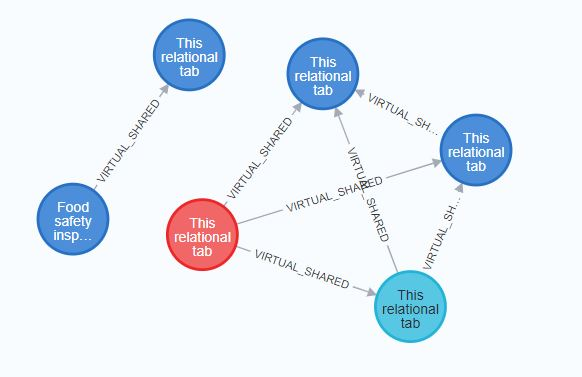
\includegraphics[width=0.65\textwidth]{IMAGES/Virtual Graph.JPG}
    \caption{Virtual Graph}
    \label{fig:Virtual Graph}
\end{figure}
By providing the LLM with the schema of the clustered Knowledge Graph, we can efficiently identify the most relevant nodes for a given query. This approach significantly reduces the graph’s size while maintaining performance comparable to the previous case involving only two tables. This approach allows for the system to scale very well as it greatly reduces the surface of the Knowledge Graph to explore, and can be stored in a persistence layer for later use, and gets reprocessed when a new CSV is fetched in our database still keeping a linear growth of complexity.

\section{Potential Improvements}

While the experiment establishes a standardized pipeline for generating structured SQL queries, several improvements can enhance its efficiency and adaptability:  

\begin{itemize}
    \item \textbf{Parallelization of LLM Prompting}: Implementing parallel processing can significantly speed up query generation by handling multiple prompts simultaneously.  
    \item \textbf{Federated Graph}: Using federated graph may allow to parallelize our system and scale it horizontally, with replication and also by keeping unrelated tables separated, removing unnecessary complexity from the workflow.
    \item \textbf{Automatic Language Detection}: Since the data sources primarily use English, querying non-English sources introduces additional complexity for the LLM in understanding both the prompt and schema. To address this, an automated language detection mechanism should be implemented. This process would:
    \begin{enumerate}
        \item Identify the language of the Open Data source.
        \item Translate the user prompt into the detected language.
        \item Generate the query in the appropriate language.
        \item Translate the final result back into the original language for consistency.
    \end{enumerate}
    \item  \textbf{Index vector store}: As the vector store increases in size the employment of specialized scalable indexes like HNSW may become more suitable, and it's worth to consider to use ACORN filtering strategy due to the correlation of the object and the querying predicate, also vector quantization may be useful in future uses.
    \item  \textbf{Automatically generated labels}: One challenge that must be tackled is the presence of automatically generated labels, which reduce significantly the sense making capabilities of the Knowledge Graph, for future applications this challenge is one of the main difficulties that must be dealt with. One possible approach is to employ an Hybrid matching between label and value based matching, between columns of matching data to improve robustness of the matching. Another possible approach is to employ a human operator to assess matching when the uncertainty is high during the matching task.
    \item \textbf{Security and query sanitation}: Security when it comes from fetching data from outside sources is always a concern to consider head on, API key must be stored in secure locations and not be put into the code or even an environment variable, if we're using containers the use of secrets is warranted. We make sure that the generated queries are sanitized and not executing an injection or other unauthorized operations. We analyze the data in order to assess that it's not tampered with, we validate and clean incoming data.
    \item \textbf{Keyword Extraction with CKAN Integration}: The system begins by extracting high-level keywords from the user’s natural language query. These keywords are used to query the CKAN open data portal via its API, leveraging available metadata for real-time dataset retrieval without prior ingestion or full indexing. If the initial keyword set is insufficient, the system iteratively refines the keywords to better match the query’s intent. Retrieved tables and metadata are stored in a structured dictionary for use in downstream processing.


\end{itemize}

These enhancements would improve both the performance and versatility of the system when handling diverse datasets.

\section{Conclusions}  

In this study, we explored the integration of Knowledge Graphs into Retrieval-Augmented Generation (RAG) to enhance the generation of SQL queries from natural language prompts. By leveraging structured relationships within a Knowledge Graph, GraphRAG provides a robust alternative to traditional vector-based retrieval methods, enabling more effective sensemaking and complex query generation. Unlike purely embedding-based retrieval approaches, which rely on semantic similarity and may struggle with structural dependencies, our framework introduces explicit relational reasoning, leading to more accurate and contextually relevant SQL query construction.  

Our experimental workflow demonstrated the feasibility of using LangGraph and Neo4j to systematically translate user queries into Cypher and SQL, ensuring both accuracy and efficiency. We implemented a hybrid retrieval strategy that combines entity matching through vector embeddings with value-based scoring, enabling more refined schema selection and join identification. This approach enhances the system’s ability to handle ambiguous or incomplete user queries by leveraging explicit graph relationships to infer missing connections. Furthermore, the multi-stage query refinement process allows for incremental improvements, ensuring that the generated SQL statements align closely with the intended query semantics.  

The evaluation of our framework over UK and Canadian OpenData datasets highlighted its effectiveness in translating natural language into precise SQL queries. We observed that the structured representation within the Knowledge Graph significantly improved the model’s ability to generate meaningful queries in complex database schemas, particularly in scenarios where conventional keyword-based retrieval failed to capture intricate table relationships. The introduction of Cypher-based retrieval prior to SQL generation facilitated improved schema sensemaking, reducing the occurrence of incorrect table joins and mismatched column references.  

While the current implementation effectively bridges natural language and structured data retrieval, several areas for future improvement remain. One key enhancement would be the parallelization of LLM prompting to reduce processing latency while maintaining high accuracy. Additionally, incorporating automatic language detection for multilingual query support could broaden the system’s applicability across diverse datasets. Further optimization of schema filtering techniques, including dynamic weighting of database elements based on query context, could further improve retrieval efficiency. Another promising avenue for exploration is the use of reinforcement learning or feedback-driven fine-tuning to iteratively enhance query generation based on user corrections and real-world usage patterns.  

Overall, this work contributes to the growing field of knowledge-driven query generation, demonstrating the potential of combining Knowledge Graphs and LLMs to simplify database interactions while maintaining expert-level accuracy. By integrating structured knowledge into the retrieval-augmented generation process, we enable more intelligent query formulation that extends beyond simple keyword matching. As AI-driven database querying continues to evolve, the fusion of structured and unstructured retrieval approaches, as demonstrated in this study, offers a promising path toward more intuitive and accessible data exploration tools.